{\small\begin{table}[H]
\centering
\begin{tabular}{lcccc}
\hline
 \textbf{Source}& \textbf{Dataset}&  &  & \textbf{Transitivity}\\ \hline
\multirow{8}{*}{Facebook} &  Politicians &   5,908  &0.0024 &  0.3011      \\
&  Companies &   14,113  & 0.0005    &     0.1532           \\
&  Athletes &   13,866  & 0.0009  &   0.1292      \\
&  News Sites &   27,917  & 0.0005  &   0.1140       \\
&  Public Figures &   11,565  & 0.0010    & 0.1666           \\
&  Artists &   50,515  &  0.0006   &    0.1140      \\
&  Government &   7,057  & 0.0036    &0.2238          \\
&  TV Shows &   3,892  & 0.0023    & 0.5906        \\\hline
 &Croatia &   54,573  &      0.0004   & 0.1146      \\
Deezer & Hungary &   47,538  & 0.0002    &      0.0929    \\
 & Romania &   41,773 &  0.0001   &       0.0752  \\
 \hline
\end{tabular}
\caption{Statistics of the datasets used in the paper for evaluation.}
\label{fig:stats}
	\vspace{-5mm}
\end{table}}
 \section{Experimental Evaluation}\label{sec:experiments}
In this section we evaluate whether the cluster quality obtained by \textit{GEMSEC} is competitive with other community detection procedures. We investigate the scalability and robustness of our method. We also explore how clustering affects the performance on downstream predictive tasks.{\small\begin{table*}
\centering
\begin{tabular}{lcccccccc}

&\multicolumn{8}{c}{\textbf{Facebook Verified Site Networks}} \\
\cline{2-9}
  & \textbf{Politicians} & \textbf{Companies} & \textbf{Athletes}   & \textbf{News Sites}   & \textbf{Public Figures} & \textbf{Artists}& \textbf{Government}& \textbf{TV Shows}   \\
\hline
\textbf{Overlap Factorization}            &&
&&& && & \0.3em]
\textbf{Fast greedy}     &&  &  & & & &&\0.3em]\hline
\textbf{DeepWalk}&&&&&&&&
\0.5em]
\textbf{GEMSEC}&&&&&&&&\0.5em]
\specialrule{.1em}{.05em}{.05em} \0.5em]
		\textbf{Smooth DeepWalk}            &&	&	&		&&	&	&		&\0.5em]
	\textbf{Smooth GEMSEC}            &	&	&	&		&&	&	&	&	\0.5em] \hline    
	\end{tabular}
		\caption{Multi-label node classification performance of the embedding extracted features on the Deezer genre likes datasets. Performance is measured by average F1 score values. Models were trained on 90\% of the data and evaluated on the remaining 10\%. Errors in the parentheses correspond to two standard deviations. \textit{GEMSEC} models consistently have good performance.}
		\label{fig:pred_perfor}
		\vspace{-5mm}
\end{table*}} \subsection{Music Genre Recommendation}
Graph embeddings are mainly used for extracting features of nodes for downstream predictive tasks. As we modified the graph embedding objective it is fair to assume that the performance on predictive problems might change due to the reformulation of the optimization problem itself. We might expect that accuracy increased or dropped by enforcing the clustering constraint. In order to investigate this we use social networks of Deezer users collected from European countries. We predict the genres of music liked by people using the embeddings. The number of distinct genres that users can like is 84 in each dataset. 

The exact experimental setup was as follows. Each graph was embedded with the standard parameter settings that gave the highest modularity. \textit{DeepWalk} embeddings used initial and final learning rate valuers such as  and . For \textit{GEMSEC} embeddings we modified the initial and final learning rates to be  and  respectively and the initial cost coefficient of the clustering was 0.1. We used logistic regression with  regularization to predict each of the labels and 90\% of the nodes were randomly selected for training. We evaluated the performance on the remaining users. The reported numbers in Table \ref{fig:pred_perfor} are mean micro, macro and weighted average F1 scores calculated from 10 experimental repetitions.

When performance is evaluated by micro-averaged F1 score we see that \textit{Smooth GEMSEC} significantly outperforms \textit{DeepWalk} on all three datasets. Precisely this performance advantage varies between 3.73\% and 8.79\%. We also see that the basic \textit{GEMSEC} is able to outperform \textit{DeepWalk} on the Hungarian and Romanian Deezer datasets when performance is measured by micro averaged F1 score. Moreover, we see that based on this metric the performance of \textit{Smooth DeepWalk} on this downstream task is as good as the performance of \textit{GEMSEC} variants. The results obtained with micro and weighted average F1 score also underpin these findings.

These results are quite interesting considering the fact that the number of naturally existing communities in these graphs might be quite different from the cluster number that we enforced in our experiment. In addition, we have evidence that introducing the clustering cost and smoothness regularization does not affect performance on the downstream predictive task adversely. On the contrary, it can increase the predictive accuracy significantly.
 \begin{figure}[H]
\centering
\begin{tikzpicture}[scale=0.4,transform shape]
\tikzset{font={\fontsize{12pt}{12}\selectfont}}
\begin{groupplot}[group style={group size=2 by 3,
	 horizontal sep=130pt, vertical sep=40pt,ylabels at=edge left},
	width=0.5\textwidth,
	height=0.5\textwidth,
	grid=major,
	grid style={dashed, gray!40},
	scaled ticks=false,
inner axis line style={-stealth}]
 \nextgroupplot[ytick={0.5,0.6,0.7,0.8,0.9},
                xtick={4,12,20,28,36,44,52,60},
	            xlabel=Clusters ,
	            ylabel=Modularity,
	            enlargelimits=0.1,
	            legend style = { column sep = 10pt, legend columns = -1, legend to name = grouplegend,}]
	
\addplot[mark=triangle*,opacity=0.8,mark options={black,fill=yellow},mark size=5pt]
coordinates {
(	4	,	0.5509225751	)
(	8	,	0.7670595551	)
(	12	,	0.8142470945	)
(	16	,	0.838909044	)
(	20	,	0.85037748	)
(	24	,	0.8491726434	)
(	28	,	0.8501187397	)
(	32	,	0.8315808317	)
(	36	,	0.8267465364	)
(	40	,	0.8081174597	)
(	44	,	0.7908403076	)
(	48	,	0.7888811936	)
(	52	,	0.7761488797	)
(	56	,	0.769325299	)
(	60	,	0.7525918277	)


	
	
};\addlegendentry{GEMSEC}\addplot[mark=diamond*,opacity=0.8,mark options={black,fill=blue},mark size=5pt]
coordinates {
(4.0,0.50971)
(8.0,0.76356)
(12.0,0.82966)
(16.0,0.85005)
(20.0,0.8551)
(24.0,0.85695)
(28.0,0.85932)
(32.0,0.85705)
(36.0,0.8549)
(40.0,0.85345)
(44.0,0.8484)
(48.0,0.84924)
(52.0,0.84552)
(56.0,0.84354)
(60.0,0.84114)


	
	
};\addlegendentry{Smooth GEMSEC}


\nextgroupplot[
ytick={0.82,0.83,0.84,0.85,0.86},
xtick={2,4,6,8,10},
xlabel=Context size,
ylabel=Modularity,
enlargelimits=0.1]

	
	\addplot[mark=triangle*,opacity=0.8,mark options={black,fill=yellow},mark size=5pt]
	coordinates {
(	1	,	0.8145516424	)
(	2	,	0.8384398568	)
(	3	,	0.8441297389	)
(	4	,	0.8492969425	)
(	5	,	0.8504032219	)
(	6	,	0.8529643002	)
(	7	,	0.8500073095	)
(	8	,	0.8526877261	)
(	9	,	0.8570090158	)
(	10	,	0.8517249459	)


		
		
	};
	\addplot[mark=diamond*,opacity=0.8,mark options={black,fill=blue},mark size=5pt]
	coordinates {
(1.0,0.8371)
(2.0,0.85481)
(3.0,0.85837)
(4.0,0.85961)
(5.0,0.85854)
(6.0,0.85801)
(7.0,0.85802)
(8.0,0.86094)
(9.0,0.86062)
(10.0,0.86055)

	
};

\nextgroupplot[
ytick={0.4,0.5,0.6,0.7,0.8},
xtick={16,32,48,64,80,96,112,128},
xlabel=Dimensions,
ylabel=Modularity, enlargelimits=0.1]
	

	
	\addplot[mark=triangle*,opacity=0.8,mark options={black,fill=yellow},mark size=5pt]
	coordinates {
(	8	,	0.8459765087	)
(	16	,	0.8505736912	)
(	24	,	0.8463623204	)
(	32	,	0.8410736967	)
(	40	,	0.8365132854	)
(	48	,	0.8251880478	)
(	56	,	0.8182187353	)
(	64	,	0.8088331064	)
(	72	,	0.7784076017	)
(	80	,	0.7395791806	)
(	88	,	0.6807693588	)
(	96	,	0.6400884371	)
(	104	,	0.5972622548	)
(	112	,	0.4983146615	)
(	120	,	0.4551573584	)
(	128	,	0.4113100453	)

		
		
	};
	\addplot[mark=diamond*,opacity=0.8,mark options={black,fill=blue},mark size=5pt]
	coordinates {
(8.0,0.85423)
(16.0,0.86018)
(24.0,0.85899)
(32.0,0.85967)
(40.0,0.85888)
(48.0,0.86115)
(56.0,0.85535)
(64.0,0.85212)
(72.0,0.84959)
(80.0,0.84712)
(88.0,0.84223)
(96.0,0.84312)
(104.0,0.83705)
(112.0,0.83163)
(120.0,0.82277)
(128.0,0.81782)



	
	};


\nextgroupplot[
/pgf/number format/precision=3,
ytick={0.844,0.848,0.852, 0.856},
	xtick={40,80,120,160},
	inner axis line style={-stealth},
	xlabel=Walk length,ylabel=Modularity, enlargelimits=0.1, legend style={at={(0.5,-0.25)},
	anchor=north,legend columns=-1},
	]
	

	
	\addplot[mark=triangle*,opacity=0.8,mark options={black,fill=yellow},mark size=5pt]
	coordinates {
(	20	,	0.8466538122	)
(	40	,	0.8487990362	)
(	60	,	0.8498392159	)
(	80	,	0.8511042033	)
(	100	,	0.8520837674	)
(	120	,	0.8520544052	)
(	140	,	0.8519378526	)
(	160	,	0.8542311674	)
		
		
	};
	\addplot[mark=diamond*,opacity=0.8,mark options={black,fill=blue},mark size=5pt]
	coordinates {

(20.0,0.85311)
(40.0,0.85419)
(60.0,0.85568)
(80.0,0.85564)
(100.0,0.85664)
(120.0,0.85636)
(140.0,0.85665)
(160.0,0.85678)


		
	};


\nextgroupplot[
/pgf/number format/precision=3,
ytick={0.8,0.82,0.84, 0.86},
xtick={0.2,0.4,0.6,0.8,1.0},
xlabel=Cluster cost coefficient,ylabel=Modularity, enlargelimits=0.1
]


\addplot[mark=triangle*,opacity=0.8,mark options={black,fill=yellow},mark size=5pt]
coordinates {
(	0.1	,	0.8503372866	)
(	0.2	,	0.8558406512	)
(	0.3	,	0.8562854305	)
(	0.4	,	0.8547253387	)
(	0.5	,	0.8501724577	)
(	0.6	,	0.8463604281	)
(	0.7	,	0.8421018614	)
(	0.8	,	0.8317438704	)
(	0.9	,	0.8077737665	)
(	1	,	0.8023874537	)

	
};
\addplot[mark=diamond*,opacity=0.8,mark options={black,fill=blue},mark size=5pt]
coordinates {

(0.1,0.85581)
(0.2,0.86094)
(0.3,0.86055)
(0.4,0.8608)
(0.5,0.8609)
(0.6,0.8596)
(0.7,0.86031)
(0.8,0.85855)
(0.9,0.85978)
(1.0,0.86019)


	
};
\nextgroupplot[
/pgf/number format/precision=3,
ytick={0.825,0.835, 0.845,0.855},
xtick={2,4,6,8,10},
xlabel=Number of radom walks,ylabel=Modularity, enlargelimits=0.1, 
]


\addplot[mark=triangle*,opacity=0.8,mark options={black,fill=yellow},mark size=5pt]
coordinates {
(	1	,	0.8412585327	)
(	2	,	0.846350781	)
(	3	,	0.8523375827	)
(	4	,	0.8530375014	)
(	5	,	0.8541093512	)
(	6	,	0.8535610696	)
(	7	,	0.8526465989	)
(	8	,	0.8518871087	)
(	9	,	0.8521070909	)
(	10	,	0.8506146118	)



};
\addplot[mark=diamond*,opacity=0.8,mark options={black,fill=blue},mark size=5pt]
coordinates {
(1.0,0.83377)
(2.0,0.84869)
(3.0,0.85877)
(4.0,0.85993)
(5.0,0.85846)
(6.0,0.86107)
(7.0,0.85988)
(8.0,0.86032)
(9.0,0.85939)
(10.0,0.86087)


};

\end{groupplot}
\node at () {\ref{grouplegend}}; 
\end{tikzpicture}
\caption{Sensitivity of cluster quality to parameter changes measured by modularity. Smoothness regularization increases the robustness of the self-clustering embedding.}\label{fig:sensi}
\vspace{-1mm}
\end{figure} \subsection{Sensitivity Analysis}\label{subsec:sensi}
The formulation of \textit{GEMSEC} involves the definition of a number of hyperparameters which affect the representation and henceforth the cluster quality. In the following experiments we test how the manipulation of hyperparameters affects the clustering performance of the introduced models. We embed the Politicians Facebook graph with the standard parameter settings while  the initial and final learning rates are set to be  and  respectively, the clustering cost coefficient is 0.1 and we perturb certain hyperparameters. In Figure \ref{fig:sensi} each data point represents the mean modularity calculated from 10 experimental repetitions. We test the sensitivity of clustering performance to cluster center number, context size, dimension number, random walk length, clustering cost coefficient and initiated random walks per source node.

Based on the experimental results we can make two main observations. First, \textit{GEMSEC} models give high quality clusterings for a wide range of parameter settings. Second, introducing smoothness regularization makes \textit{GEMSEC} more robust to hyperaparameter changes when performance is evaluated by cluster quality. Specifically, we observe that increasing the cluster number above 30 decreases slightly the average modularity. In case of the non smooth model the decrease in cluster quality is quite considerable.

 We conclude that increasing the context size, the length of truncated random walks and the number of random walks per source node above a certain threshold has only marginal effect on the community detection performance. Interestingly, we also have empirical evidence for the node capture phenomenon --- if the clustering cost coefficient is too high vanilla \textit{GEMSEC} has a poor clustering performance. Finally, there is strong evidence that both \textit{GEMSEC} and \textit{Smooth GEMSEC} perform poorly when the number of dimensions used to create the embedding is high.
 
\subsection{Smoothness Regularization Strategies}
As we have seen the introduction of smoothness regularization can boost the clustering performance considerably. In Subsection \ref{subsec:reg} we defined different strategies for weighting edges in the smoothness regularization cost. It is presumed that these strategies work well with different values of the regularization coefficient. In this set of experiments we manipulate the regularization coefficient and look at the modularity under the earlier defined edge distance weighting strategies. We create embeddings of the Facebook Politcians graph with the parameter settings used in Subsection \ref{subsec:sensi} and we plotted on Figure \ref{fig:regul_regimes} the mean modularity based on 10 experimental repetitions.
\begin{figure}[h!]
\centering
\begin{tikzpicture}[scale=0.4,transform shape]
\tikzset{font={\fontsize{12pt}{12}\selectfont}}
\begin{groupplot}[group style={group size=2 by 1,
	 horizontal sep=130pt, vertical sep=60pt,ylabels at=edge left},
	width=0.5\textwidth,
	height=0.5\textwidth,
	grid=major,
	grid style={dashed, gray!40},
	scaled ticks=false,
inner axis line style={-stealth}]
 \nextgroupplot[xtick={-13,-11,-9,-7,-5,-3,-1},
                ymin=0,
                ytick={0,0.2,0.4,0.6,0.8},
	            xlabel= Regularization coefficient,
	            ylabel=Modularity,
	            enlargelimits=0.1,
	            legend style = { column sep = 10pt, legend columns = -1, legend to name = grouplegend,},title={Smooth DeepWalk}]
	
\addplot[mark=*,opacity=0.8,mark options={black,fill=blue},mark size=3pt]
	coordinates {
(-13.0,0.48941)
(-12.0,0.48989)
(-11.0,0.51354)
(-10.0,0.55782)
(-9.0,0.64134)
(-8.0,0.69933)
(-7.0,0.74316)
(-6.0,0.78914)
(-5.0,0.81172)
(-4.0,0.8219)
(-3.0,0.83249)
(-2.0,0.83639)
(-1.0,0.83552)
(0.0,0.8368)


};\addlegendentry{Normalized overlap}
	
\addplot[mark=square*,opacity=0.8,mark options={black,fill=green},mark size=3pt]
coordinates {
(-13.0,0.75866)
(-12.0,0.79056)
(-11.0,0.80793)
(-10.0,0.80461)
(-9.0,0.81898)
(-8.0,0.82911)
(-7.0,0.81994)
(-6.0,0.76846)
(-5.0,0.61143)
(-4.0,0.55946)
(-3.0,0.42839)
(-2.0,0.22544)
(-1.0,0.16988)
(0.0,0.12301)



	
};\addlegendentry{Overlap}

\addplot[mark=triangle*,opacity=0.8,mark options={black,fill=orange},mark size=5pt]
coordinates {
(-13.0,0.5121)
(-12.0,0.56906)
(-11.0,0.68521)
(-10.0,0.74124)
(-9.0,0.80371)
(-8.0,0.83624)
(-7.0,0.83897)
(-6.0,0.84609)
(-5.0,0.84295)
(-4.0,0.84281)
(-3.0,0.82439)
(-2.0,0.787)
(-1.0,0.6578)
(0.0,0.63588)


	
	
};\addlegendentry{Unit}
\addplot[mark=*,opacity=0.8,mark options={black,fill=red},mark size=3pt]
coordinates {
(-13.0,0.51159)
(-12.0,0.5057)
(-11.0,0.5958)
(-10.0,0.66765)
(-9.0,0.74695)
(-8.0,0.78553)
(-7.0,0.81164)
(-6.0,0.82022)
(-5.0,0.82246)
(-4.0,0.8336)
(-3.0,0.83912)
(-2.0,0.83792)
(-1.0,0.81876)
(0.0,0.72933)


	
	
	
	
};\addlegendentry{Min Normalized Overlap}

 \nextgroupplot[xtick={-13,-11,-9,-7,-5,-3,-1},
 ytick={0.2,0.4,0.6,0.8},
 ymin=0.2,
 xlabel= Regularization coefficient,
 ylabel=Modularity,
 enlargelimits=0.1,
 legend style = { column sep = 10pt, legend columns = -1, legend to name = grouplegend,},title={Smooth GEMSEC}]
 
 \addplot[mark=*,opacity=0.8,mark options={black,fill=blue},mark size=3pt]
 coordinates {
(-13.0,0.84291)
(-12.0,0.84766)
(-11.0,0.84745)
(-10.0,0.84684)
(-9.0,0.84794)
(-8.0,0.84979)
(-7.0,0.8499)
(-6.0,0.85319)
(-5.0,0.85476)
(-4.0,0.85772)
(-3.0,0.85546)
(-2.0,0.85221)
(-1.0,0.85016)
(0.0,0.84872)


};\addlegendentry{Jaccard's coefficient}
 
 \addplot[mark=square*,opacity=0.8,mark options={black,fill=green},mark size=3pt]
 coordinates {
(-13.0,0.84819)
(-12.0,0.84927)
(-11.0,0.84902)
(-10.0,0.85428)
(-9.0,0.85299)
(-8.0,0.84803)
(-7.0,0.8423)
(-6.0,0.8483)
(-5.0,0.83694)
(-4.0,0.80444)
(-3.0,0.68608)
(-2.0,0.51881)
(-1.0,0.29746)
(0.0,0.23375)

};\addlegendentry{Neighborhood overlap}
 
 \addplot[mark=triangle*,opacity=0.8,mark options={black,fill=orange},mark size=5pt]
 coordinates {
(-13.0,0.84484)
(-12.0,0.8481)
(-11.0,0.85056)
(-10.0,0.84869)
(-9.0,0.8543)
(-8.0,0.85902)
(-7.0,0.86107)
(-6.0,0.8593)
(-5.0,0.85685)
(-4.0,0.85398)
(-3.0,0.85529)
(-2.0,0.85264)
(-1.0,0.84931)
(0.0,0.84067)

 };\addlegendentry{Unit}
 \addplot[mark=*,opacity=0.8,mark options={black,fill=red},mark size=3pt]
 coordinates {
(-13.0,0.84827)
(-12.0,0.84426)
(-11.0,0.84602)
(-10.0,0.85055)
(-9.0,0.85025)
(-8.0,0.85196)
(-7.0,0.85522)
(-6.0,0.85753)
(-5.0,0.85541)
(-4.0,0.85549)
(-3.0,0.84935)
(-2.0,0.84996)
(-1.0,0.83888)
(0.0,0.82216)

 };\addlegendentry{Minimum normalized overlap}
\end{groupplot}
\node at () {\ref{grouplegend}}; 
\end{tikzpicture}
\caption{Sensitivity of cluster quality to smoothness regularization coefficient on the Facebook politicians network. \textit{Smooth GEMSEC} shows a stronger robustness to regularization coefficient changes.}\label{fig:regul_regimes}
\vspace{-2mm}
\end{figure} 
The main insights based on the experiments are summarized as follows. The clustering performance of \textit{DeepWalk} is more sensitive to the regularization coefficient than that of \textit{GEMSEC}. We observe that \textit{GEMSEC} has high quality results with nearly every possible weighting strategy and setting of the regularization coefficient.  Moreover, when the coefficient is too high the neighborhood overlap, minimum normalized overlap and unit weighting has considerable adverse effects on the clustering performance of \textit{DeepWalk}. Finally, the clustering performance under the standard setting of the regularization coefficient seems to be optimal for both models.

\subsection{Robustness to Perturbation}
In a number of settings the graph that we observe contains noisy edges or edges among vertices are not present. In a social network people who do not know each other might share an edge or conversely users who do know someone decide not to be linked on purpose. As such applications are highly relevant for real-world applications we will test the robustness of \textit{GEMSEC} to these types of perturbations and compare it to the \textit{DeepWalk} variants. 

Utilizing the Facebook Politicians graph we create synthetic graphs where a given fraction of nodes is randomly removed or added while the number of connected components is unchanged. Using these synthetic graphs we created a clustering of nodes and evaluated the modularity on the original graph. We used the hyperparameter settings from Subsection \ref{subsec:sensi} and each experiment was repeated 10 times. The plots on Figure \ref{fig:attenuation} report mean modularity and error bars correspond to two standard deviations.
\begin{figure}[h!]
	\centering
	\begin{tikzpicture}[scale=0.7,transform shape]
	\tikzset{font={\fontsize{8pt}{12}\selectfont}}
	\begin{groupplot}[group style={group size=1 by 1,
		horizontal sep=60pt, vertical sep=60pt,ylabels at=edge left},
	width=0.9\textwidth,
	height=0.9\textwidth,
  x=2.5cm,
  ytick={0.78,0.8,0.82,0.84,0.86},
  height=5cm,
  enlargelimits=0.15,
  xtick={1,2,3,4},
  xticklabels={-20\%, -10\%, 10\%, 20\%},
  grid=major,
  ybar]
 \nextgroupplot[title = {Politicians dataset},  legend style = { column sep = 10pt, legend columns = -1, legend to name = groupl,}]
\addplot[area legend,
fill=red!70,
pattern=north west lines,
pattern color=red!70,
draw=black,
point meta=y,
every node near coord/.style={inner ysep=5pt},
error bars/.cd,
y dir=both,
y explicit
] 
table [y error=error] {
	x   y           error    label
	1	0.8244227272	0.0070519497
	2	0.8282159522	0.0128103686
	3	0.789531333	0.0134271832
	4	0.7788797369	0.0071791417
	
};\addlegendentry{DeepWalk}

\addplot[
area legend,
fill=red!70,
pattern=grid,
pattern color=green!50,
draw=black,
point meta=y,
every node near coord/.style={inner ysep=5pt},
error bars/.cd,
y dir=both,
y explicit
] 
table [y error=error] {
	x   y           error    label
	1	0.8495472957	0.0079266963
	2	0.8530512786	0.0062603507
	3	0.8345134589	0.0078587824
	4	0.8250597715	0.0089327901
	
};\addlegendentry{Smooth DeepWalk}
\addplot[
area legend,
fill=blue!70,
draw=black,
pattern=north east lines,
pattern color=orange!70,
point meta=y,
every node near coord/.style={inner ysep=5pt},
error bars/.cd,
y dir=both,
y explicit] 
table [y error=error] {
	x   y           error    
1	0.8407723969	0.0124382537
2	0.8426889237	0.0142236843
3	0.8153349833	0.0106964732
4	0.7978803752	0.014986018

};\addlegendentry{GEMSEC}

\addplot[
area legend,
fill=blue!25,
draw=black,
point meta=y,
every node near coord/.style={inner ysep=5pt},
error bars/.cd,
y dir=both,
y explicit
] 
table [y error=error] {
	x   y           error    label
1	0.85265345	0.0072666422
2	0.8536476278	0.0062535701
3	0.8417975179	0.0050057167
4	0.8280207633	0.0078725095
	
};\addlegendentry{Smooth GEMSEC}
 
 \draw ({rel axis cs:0,0}|-{axis cs:0,0}) -- ({rel axis cs:1,0}|-{axis cs:0,0});

 \end{groupplot}
 \node at () {\ref{groupl}}; 
\end{tikzpicture}
\caption{Sensitivity of cluster quality to randomized edge removal and addition measured by modularity. Smoothness regularization increases robustness to edge addition.}\label{fig:attenuation}
\vspace{-2mm}
\end{figure} 
First, we can observe that all of the models are quite robust to edge removal --- we see little difference between the modularity values when we increased the fraction of removed edges from 10\% to 20\%. On the contrary the addition of edges that are non-existent in the original graph has a considerable adverse effect on clustering performance. Second, we see that the use of smoothness regularization with Jaccard's index weighting mitigates this effect. This is due to the fact that noisy edges between randomly selected nodes are expected to have a zero neighborhood overlap. Because of this, for noise edges we do not have a constraint on making representations to be similar. Finally, it should be considered that even when we add a considerable amount of edges randomly we are able to perform comparably to the baselines.

\subsection{Scalability}
As scalability is an important aspect in real world applications we also investigated the scalability of our procedure. The quantity of interest was the time needed to do a single training epoch as the sampling procedure and the feature extraction is equivalent to that of \textit{DeepWalk} (assuming that the regularization weights are pre-calculated). Our experiments were done on Erdos-Renyi graphs with a fixed average degree of 20. We created embeddings of this graph with both \textit{DeepWalk} and \textit{GEMSEC} variants and we used the baseline parameter settings to create embeddings. We calculated mean optimization runtime in seconds per epoch based on ten epochs. The logarithms of these averages as a function of the log node number are plotted on Figure \ref{fig:performance}.
\begin{figure}[!h]
\centering
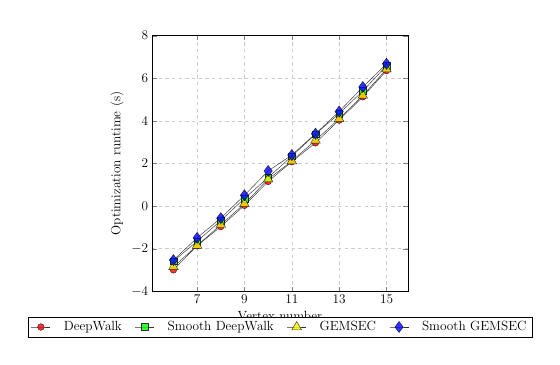
\begin{tikzpicture}[scale=0.4,transform shape]
\tikzset{font={\fontsize{12pt}{12}\selectfont}}
\begin{axis}[
width=0.8\textwidth,
height=0.8\textwidth,
grid=major,
grid style={dashed, gray!40},
scaled ticks=false,
inner axis line style={-stealth}
yticklabels={-3,-1,...,7},
ymin=-3,
ymax=7,
xtick={7,9,11,13,15},
legend style = {at={(0.5,-0.1)},anchor=north, column sep = 10pt,legend columns = -1},
xlabel= Vertex number,
ylabel= Optimization runtime (s),
 enlargelimits=0.1, 
]

\addplot[mark=*,opacity=0.8,mark options={black,fill=red},mark size=3pt]
coordinates {

	(6,-2.993)
	(7,-1.861)
	(8,-0.959)
	(9,0.034)
	(10,1.157)
	(11,2.083)
	(12,2.968)
	(13,4.035)
	(14,5.131)
	(15,6.359)
	
	
};\addlegendentry{DeepWalk}

\addplot[mark=square*,opacity=0.8,mark options={black,fill=green},mark size=3pt]
coordinates {

(6,-2.585)
(7,-1.649)
(8,-0.68)
(9,0.359)
(10,1.34)
(11,2.343)
(12,3.375)
(13,4.344)
(14,5.4)
(15,6.595)


	
};\addlegendentry{Smooth DeepWalk}

\addplot[mark=triangle*,opacity=0.8,mark options={black,fill=yellow},mark size=5pt]
coordinates {

(6,-2.852)
(7,-1.851)
(8,-0.874)
(9,0.108)
(10,1.265)
(11,2.112)
(12,3.087)
(13,4.098)
(14,5.193)
(15,6.425)

	
};\addlegendentry{GEMSEC}
\addplot[mark=diamond*,opacity=0.8,mark options={black,fill=blue},mark size=5pt]
coordinates {

	(6,-2.535)
	(7,-1.49)
	(8,-0.566)
	(9,0.508)
	(10,1.648)
	(11,2.395)
	(12,3.397)
	(13,4.437)
	(14,5.589)
	(15,6.679)
	
};\addlegendentry{Smooth GEMSEC}



\end{axis}
\end{tikzpicture}
\caption{Sensitivity of optimization runtime to graph size measured by seconds. Our proposed models' optimization has linear runtime complexity in the number of nodes.}\label{fig:performance}
\vspace{-2mm}
\end{figure} 
Most importantly, based on Figure \ref{fig:performance} we can conclude that doubling the size of the graph doubles the time needed for optimizing \textit{GEMSEC}. The linear nature of the proposed algorithm is well demonstrated by the figure. We also observe that learning the clustering and embedding jointly increases optimization time, which was expected. Besides this, the presence of smoothness regularization also inflates the time needed for optimization, but each of the smooth algorithms scales linearly with the number of vertices.